\documentclass[journal,10pt,twocolumn]{article}
\usepackage{graphicx}
\usepackage[margin=0.5in]{geometry}
\usepackage[cmex10]{amsmath}
\usepackage{array}
\usepackage{booktabs}
\usepackage{mathtools}
\title{\textbf{Optimization Assignment - 1}}
\author{T.manasareddy}
\date{September 2022}


\providecommand{\norm}[1]{\left\lVert#1\right\rVert}
\providecommand{\abs}[1]{\left\vert#1\right\vert}
\let\vec\mathbf
\newcommand{\myvec}[1]{\ensuremath{\begin{pmatrix}#1\end{pmatrix}}}
\newcommand{\mydet}[1]{\ensuremath{\begin{vmatrix}#1\end{vmatrix}}}
\providecommand{\brak}[1]{\ensuremath{\left(#1\right)}}
\providecommand{\lbrak}[1]{\ensuremath{\left(#1\right.}}
\providecommand{\rbrak}[1]{\ensuremath{\left.#1\right)}}
\providecommand{\sbrak}[1]{\ensuremath{{}\left[#1\right]}}

\begin{document}

\maketitle
\paragraph{\textit{Problem Statement} - A rectangular sheet of tin 45cm by 24cm is to be made into a box without top,by cutting off square from each corner and floding up the flaps.What should be the side of the square to be cut off so that the volume of the box is maximum}

\section*{\large Solution}
\subsection*{\normalsize Monomial approximation}
Let $h$ be the side of the square removed. Let $l$ and $b$ be the length and breadth of the box. Due to the construction, $h$ is the height of the box. The volume of the box can be expressed as
\begin{align}
	V = lbh
\end{align}
where
\begin{align}
	\label{eq:con_eq1}
	l = 45 - 2h\\
	\label{eq:con_eq2}
	b = 24 - 2h
\end{align}
Since l and h are positive, from \eqref{eq:con_eq1} and \eqref{eq:con_eq2} we get
\begin{align}
	h <= \min(22.5, 12)\\
	\implies h <= 12
	\label{eq:lt_eq1}
\end{align}
The problem can be formulated as
\begin{align}
	\label{eq:prob_std}
	P = \max_{l,b,h}lbh\\
	\label{eq:con_eq_st1}
	l + 2h = 45\\
	\label{eq:con_eq_st2}
	b + 2h = 24\\
	\label{eq:lt_eq_std}
	h <= 12
\end{align}
The above formulation is not a geometric programming problem since the equality constraints \eqref{eq:con_eq_st1} and \eqref{eq:con_eq_st2} are posynomials. To convert the problem into a geometric programming problem, we approximate the posynomials in the equality constraints as monomials using
\begin{align}
	\label{eq:mono_approx}
	f(w) \approx f(x)\prod_{i=1}^{n}\brak{\frac{w_i}{x_i}}^{a_i}
\end{align}
where
\begin{align}
	a_i = \frac{x_i}{f(x)}\frac{\partial{f}}{\partial{x_i}}
\end{align}
Approximating \eqref{eq:con_eq_st1} and \eqref{eq:con_eq_st2} as $f(l,b,h)$ and $g(l,b,h)$ respectively using \eqref{eq:mono_approx}, the problem is expressed as
\begin{align}
	P = \max_{l,b,h}lbh\\
	f(l,b,h) = 45\\
	g(l,b,h) = 24\\
	h >= \frac{h_k}{1+\Delta}\\
	h <= \min((1+\Delta)h_k, 12)
\end{align}
Where $h_k$ is the current guess of $h$ and $\Delta$ is the parameter to determine the trust region around $h_k$ where the approximation in \eqref{eq:mono_approx} holds valid.
The above formulation can be iterated till the problem converges at a local maximum. Taking $n = 100$ and $\Delta = 0.005$, the optimal solution obtained using cvxpy is
\begin{align}
	\boxed{V_{max} = 660.91}\\
	\boxed{h = 0.664331}
\end{align}
\subsection*{\normalsize Gradient descent}
Let $x$ be the side of each square removed. The volume of the box can be expressed as
\begin{align}
	\label{eq:vol_varx}
	f(x) = (45-2x)(24-2x)x\\
	\implies f(x) = 4x^3-138x^2+1080x
	\label{eq:cubic_exp}
\end{align}
The polynomial in \eqref{eq:cubic_exp} has roots at $x = 0$, $x = 12$ and $x = 22.5$. Since the coefficient of $x^3$ is positive and the roots are distinct, it can be concluded that there exists a local maximum between $x = 0$ and $x = 22.5$. This can be seen in Figure \ref{fig:graph_fx}.
Using gradient ascent method we can find its maxima in the interval $\mathbf{[}0,1.5\mathbf{]}$,
    \begin{align}
        x_{n+1} &= x_n + \alpha \nabla f(x_n) \\
        \implies x_{n+1} &= x_n + \alpha \brak{12x_n^2-276x_n+1080}
    \end{align}
    
Taking $x_0=0.5,\alpha=0.001$ and precision = 0.00000001, values obtained using python are:
    
    \begin{align}
        \boxed{\text{Maxima} = 660.91}\\
        \boxed{\text{Maxima Point} = 0.666666}
    \end{align}

\begin{figure}[t]
	\centering
	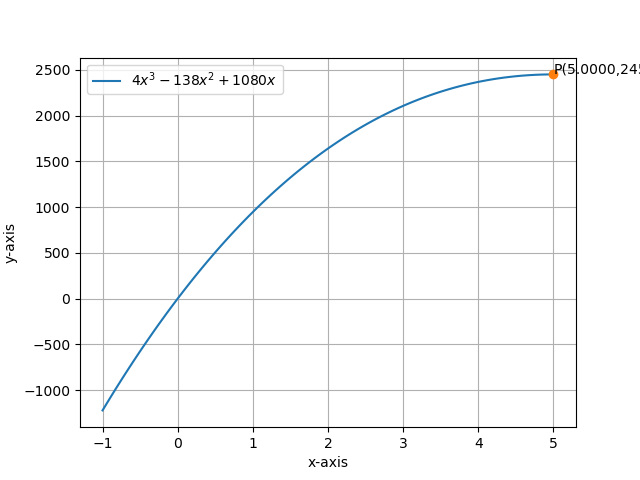
\includegraphics[width=1\columnwidth]{fig1.png}
	\caption{Graph of $f(x)$ in \eqref{eq:cubic_exp}}
	\label{fig:graph_fx}
\end{figure}

\end{document}